\documentclass{ximera}
\title{Riemann Sums}
\begin{abstract}
\end{abstract}
\begin{document}
\maketitle
\begin{javascript}
 caseInsensitive = function(a,b) {
    return a.toLowerCase() == b.toLowerCase();
  };
\end{javascript}
\begin{dialogue}
\item[Dylan] Hey Julia, can you help me with this problem?
\item[Julia] Yeah, of course! What do you need?
\item[Dylan] I'm supposed to approximate area under a curve, and I don't really see what to do.
\item[Julia] Actually, that's pretty easy! We'll just use Riemann sums.
\end{dialogue}

\section{Introduction}
Riemann sums are a method of approximating area under a curve, we will look at three varieties; left, right, and midpoint.

\begin{image}
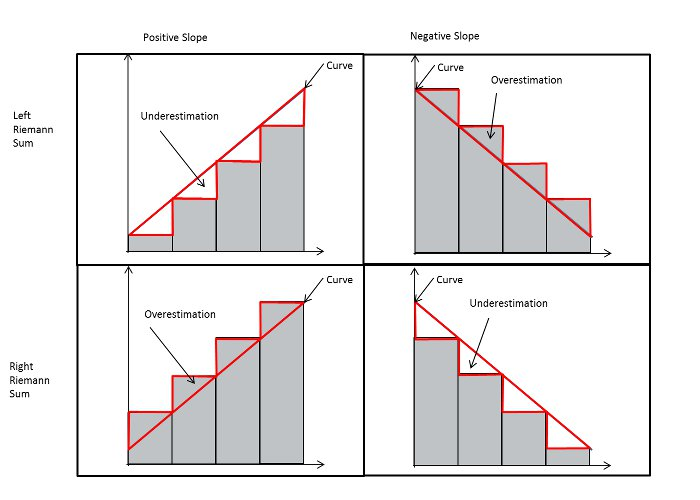
\includegraphics{Table}
\end{image}
\begin{center}
\textit{Obtained from \href{http://mathforum.org/mathimages/index.php/Riemann_Sums}{mathforum.org}}
\end{center}


To create Riemann sums, you simply pick a number of desired subintervals, and then evenly divide the interval to produce the desired number. From here, we choose the height of what will be our rectangles differently for each version:
\begin{itemize}
\item{\textbf{Left Riemann Sum:} The height is calculated using the left endpoint of the subinterval.}
\item{\textbf{Right Riemann Sum:} The height is calculated using the right endpoint of the subinterval.}
\item{\textbf{Midpoint Riemann Sum:} The height is calculated using the midpoint of the subinterval.}
\end{itemize}

From here, we simply add the area of each rectangle to produce the area under the curve.

If we are approximating area with $n$ rectangles, then
\begin{align*}
  \text{Area} &\approx \sum_{k=1}^n (\text{height of $k$th rectangle})\times(\text{width of $k$th rectangle}) \\
  &=\sum_{k=1}^n  f(x_k^*)\Delta x \\
  &=  f(x_1^*)\Delta x +  f(x_2^*)\Delta x +   f(x_3^*)\Delta x + \dots +   f(x_n^*)\Delta x.
\end{align*}
\begin{definition}
  A sum of the form:
  \[
  \sum_{k=1}^n  f(x_k^*)\Delta x  = f(x_1^*)\Delta x +  f(x_2^*)\Delta x + \dots +   f(x_n^*)\Delta x
  \]
  is called a \textbf{Riemann sum}.
\end{definition}

\section{Increasing, Concave Up}
Consider the function $x^2$ on the interval [1, 6].
\[
\graph[xmin=-1,xmax=7,ymin=-1,ymax=40,height=400]{x^2}
\]


\begin{question}
The following qustion shows how to compute the Riemann sums using Sage cells, you will need to mimic this process in further questions so be sure to read the Sage code and understand how it represents the equation for Riemann sums.


The left Riemann sum.

\begin{onlineOnly}
\begin{sageCell}
f(x) = x^2
a=1.0
b=6.0
n=6
Dx=(b-a)/n
rsum=sum([f(a+i*Dx)*Dx for i in range(n)])
print rsum
\end{sageCell}
\end{onlineOnly}
What did you get for the left Reimann sum from evaluating the above Sage cell?
$\answer{57.6620370370370}$


The right Riemann sum.

\begin{onlineOnly}
\begin{sageCell}
f(x) = x^2
a=1.0
b=6.0
n=6
Dx=(b-a)/n
rsum=sum([f(a+(i+1)*Dx)*Dx for i in range(n)])
print rsum
\end{sageCell}
\end{onlineOnly}
What did you get for the right Reimann sum from evaluating the above Sage cell?
$\answer{86.8287037037037}$
\begin{feedback}
Notice the change in the second to last line between the code for left and right Riemann sums.
\end{feedback}

The midpoint Riemann sum.
\begin{onlineOnly}
\begin{sageCell}
f(x) = x^2
a=1.0
b=6.0
n=6
Dx=(b-a)/n
rsum=sum([f(a+(i+0.5)*Dx)*Dx for i in range(n)])
print rsum
\end{sageCell}
\end{onlineOnly}
What did you get for the midpoint Reimann sum from evaluating the above Sage cell?
$\answer{71.3773148148148}$

Compute the integral numerically by evaluating the following Sage cell. Which of these estimates was most accurate? Show the percent error for each type of Riemann sum, rounding to two decimal places.

\begin{onlineOnly}
\begin{sageCell}
integral(x^2,x,0,6)
\end{sageCell}
\end{onlineOnly}

Most Accurate:
\begin{multipleChoice}
\choice{Left Riemann Sum}
\choice{Right Riemann Sum}
\choice[correct]{Midpoint Riemann Sum}
\end{multipleChoice}
Left Percent Error: $\answer{19.91}$\%

Middle Percent Error: $\answer{0.86}$

Right Percent Error: $\answer{20.60}$
\end{question}

\section{Decreasing, Concave Up}
\begin{question}
Consider the function $x^2$ on the interval [-7, 0].

\[
\graph[height=400,xmin=-8,xmax=1,ymin=-1,ymax=55]{x^2}
\]

Calculate the following Riemann sums by modifying the code provided in the first question to have seven subintervals and reflect the new endpoints.

The left Riemann sum.

\begin{onlineOnly}
\begin{sageCell}

\end{sageCell}
\end{onlineOnly}

$\answer{140}$

The right Riemann sum.

\begin{onlineOnly}
\begin{sageCell}

\end{sageCell}
\end{onlineOnly}

$\answer{91}$

The midpoint Riemann sum.

\begin{onlineOnly}
\begin{sageCell}

\end{sageCell}
\end{onlineOnly}

$\answer{113.75}$

Compute the integral numerically. Which of these estimates was most accurate? Show the percent error for each type of Riemann sum, rounding to two decimal places.

\begin{onlineOnly}
\begin{sageCell}

\end{sageCell}
\end{onlineOnly}

Most Accurate:
\begin{multipleChoice}
\choice{Left Riemann Sum}
\choice{Right Riemann Sum}
\choice[correct]{Midpoint Riemann Sum}
\end{multipleChoice}
Left Percent Error: $\answer{22.45}$\%

Middle Percent Error: $\answer{0.51}$\%

Right Percent Error: $\answer{20.41}$\%
\end{question}

\section{Increasing, Concave Down}
\begin{question}
\begin{hint}
Add .n() right after rsum to get a clean numerical approximation.
\end{hint}
Consider the function $\sin(x)$ on the interval [0,$\frac{\pi}{2}$].

\[
\graph[xmin=-.5,xmax=2,ymin=-1.5,ymax=1.5,height=400]{sin(x)}
\]

Calculate the following Riemann sums by modifying the code provided in the first question to have four subintervals and reflect the new endpoints and new function.

The left Riemann sum.

\begin{onlineOnly}
\begin{sageCell}

\end{sageCell}
\end{onlineOnly}

$\answer{0.790766260123413}$

The right Riemann sum.

\begin{onlineOnly}
\begin{sageCell}

\end{sageCell}
\end{onlineOnly}

$\answer{1.18346534182214}$

The midpoint Riemann sum.

\begin{onlineOnly}
\begin{sageCell}

\end{sageCell}
\end{onlineOnly}

$\answer{1.00645454279956}$

Compute the integral numerically. Which of these estimates was most accurate? Show the percent error for each type of Riemann sum, rounding to two decimal places.

\begin{onlineOnly}
\begin{sageCell}

\end{sageCell}
\end{onlineOnly}

Most Accurate:
\begin{multipleChoice}
\choice{Left Riemann Sum}
\choice{Right Riemann Sum}
\choice[correct]{Midpoint Riemann Sum}
\end{multipleChoice}

Left Percent Error: $\answer{20.92}$\%

Middle Percent Error: $\answer{0.65}$\%

Right Percent Error: $\answer{18.35}$\%
\end{question}


\section{Decreasing, Concave Down}
\begin{question}
Consider the function $\cos(x)$ on the interval [0, $\frac{\pi}{2}$].

\[
\graph[xmin=-.5,xmax=2,ymin=-1.5,ymax=1.5,height=400]{cos(x)}
\]

Calculate the following Riemann sums by modifying the code provided in the first question to have four subintervals and reflect the new endpoints and new function.

The left Riemann sum.

\begin{onlineOnly}
\begin{sageCell}

\end{sageCell}
\end{onlineOnly}

$\answer{1.18346534182214}$

The right Riemann sum.

\begin{onlineOnly}
\begin{sageCell}

\end{sageCell}
\end{onlineOnly}

$\answer{0.790766260123413}$

The midpoint Riemann sum.

\begin{onlineOnly}
\begin{sageCell}

\end{sageCell}
\end{onlineOnly}

$\answer{1.00645454279956}$

Compute the integral numerically. Which of these estimates was most accurate? Show the percent error for each type of Riemann sum, rounding to two decimal places.

\begin{onlineOnly}
\begin{sageCell}

\end{sageCell}
\end{onlineOnly}

Most Accurate:
\begin{multipleChoice}
\choice{Left Riemann Sum}
\choice{Right Riemann Sum}
\choice[correct]{Midpoint Riemann Sum}
\end{multipleChoice}
Left Percent Error: $\answer{18.35}$\%

Middle Percent Error: $\answer{0.65}$\%

Right Percent Error: $\answer{20.92}$\%
\end{question}

\begin{dialogue}
\item[Dylan] That's cool! Thanks Julia!
\item[Julia] No problem!
\item[Dylan] I wish I could make the sums more accurate though... some of them are pretty far off.
\item[James] I think if you put your mind to it you could Dylan!
\item[Julia and Dylan] James! You're late to class!
\item[James] Haha no problem, I love helpi... that's not the point! Listen, just use sum notation, and try to make infinitely many subintervals. If you can do that, you'll have an accurate area.
\end{dialogue}
\begin{question}

\begin{hint}
Think of the start of the interval as $a$ and the end as $b$.
\end{hint}

How would you represent the width of each rectangle when divided into $n$ subintervals?

\begin{multipleChoice}
\choice{$\frac{b+a}{2}$}
\choice{$\frac{b-a}{2}$}
\choice[correct]{$\frac{b-a}{n}$}
\choice{$\frac{n}{b-a}$}
\end{multipleChoice}

\begin{hint}
As $n$ grows larger, will the rectangle be wider than a single point? What does that tell you about the height?
\end{hint}

How would you represent the height of each rectangle when divided into $n$ subintervals?

\begin{multipleChoice}
\choice{$f(x)$}
\choice{$f(x_b)-f(x_a)$}
\choice{$\frac{f(x_b)-f(x_a)}{2}$}
\choice{$\sum_{i=a}^b f(x_i)$}
\end{multipleChoice}

How could you use sigma notation to represent the area under the curve from $i = 1$ to $n$, as $n$ approaches infinity?

\begin{multipleChoice}
\choice[correct]{$\lim_{n\to \infty} \sum_{i=1}^n$}
\choice{$\lim_{n\to 0} \sum_{i=1}^n$}
\choice{$\lim_{n\to \infty} \sum_{i=1}^\infty$}
\choice{$\sum_{i=1}^n \lim_{n \to \infty}$}
\end{multipleChoice}

\end{question}
\begin{dialogue}
\item[Julia] Wow, that's just as accurate as asking our computers!
\item[James] That's right Julia! You just found the integral of a function, with just a little guidance!
\item[Julia and Dylan] Wow! Thanks James!
\end{dialogue}

\section{In Summary}
We've learned a lot about Riemann sums today, and even the formula for a definite integral! So let's recap:
\begin{definition}
A \textbf{Riemann sum} comes in three types, all of which first divide an interval into a number of subintervals:
\begin{enumerate}
\item{\textbf{Left endpoint Riemann sums} use the left endpoint of the subinterval to approximate the area.}
\item{\textbf{Right endpoint Riemann sums} use the right endpoint of the subinterval to approximate the area.}
\item{\textbf{Midpoint Riemann sums} use the midpoint of the subinterval to approximate the area.}
\end{enumerate}
Following this, the area of each rectangle is added to approximate the area under the curve.
\end{definition}

\begin{itemize}
\item{The formula for the definite integral is $$\displaystyle \int_a^b f(x) = \lim_{n\to\infty} \sum_{i=1}^n f(x) \cdot \frac{a-b}{n}$$where $a$ and $b$ are the endpoints of the interval.}
\end{itemize}
\pagebreak
\end{document}